\documentclass[runningheads]{llncs}
\usepackage{graphicx}

\begin{document}
	\title{CS32420 Angry Blobs - Project Report}
	\author{Rhys Evans}
	\institute{Department of Computer Science,\\ Aberystwyth University, \\Aberystwyth\\
	\email{rhe24@aber.ac.uk}}
	\maketitle
	
	\begin{abstract}
		The basis of this project was to create a simple projectile launching game using three.js~\cite{ref_threejs} and physijs~\cite{ref_physijs}. The game is called 'Angry Blobs', it is a 'best of three' competition between a human player and an AI player. The two players each take a turn firing a projectile at a structure of blocks. A score is awarded each turn based on the success of the hit, at the end of the game a winner is decided based on the scores. The purpose of the project is to practically apply and demonstrate an understanding of graphics and game development techniques and principles. URLs to a working version of the game can be found below:\\ \url{http://users.aber.ac.uk/rhe24/angryblobs} \\ \url{http://code.rhysevans.xyz/angryblobs}
	\end{abstract}
	
	\newpage
	\section{Functionalities} \label{functionalities}
	This section will briefly describe the game's key functionalities, without going into specific detail about their implementation.
	\subsection{Screens}
	There are 3 screens that are displayed throughout the game: start screen, game screen, end screen. The start screen contains a brief 'how to' for the user to understand the game, a difficulty option for the AI opponent and a start button to begin the game (see Fig.~\ref{start-screen}). The game screen contains the three.js~\cite{ref_threejs} scene and the necessary UI components (score display, round and turn display, end game button). Lastly, the end screen contains a win/lose label, a breakdown of the scores and two buttons: Home and Restart.
	\begin{figure}
		\centering
		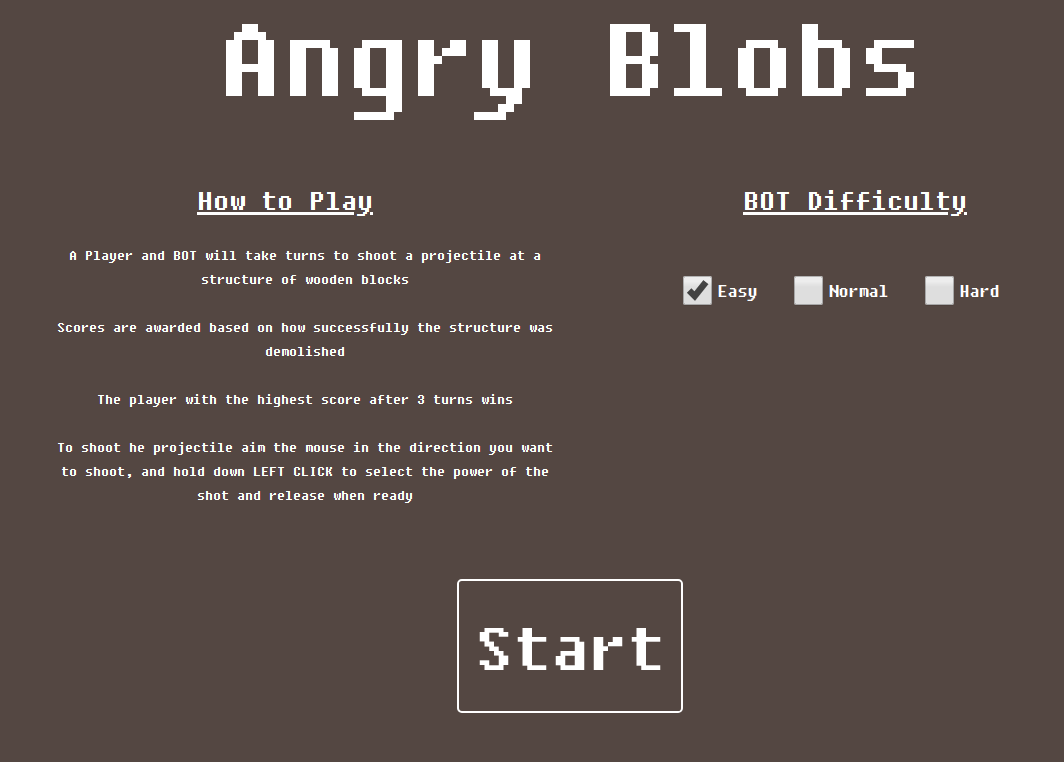
\includegraphics[width=\textwidth]{./img/start-screen.png}
		\caption{The start screen}
		\label{start-screen}
	\end{figure}
	\subsection{Firing the Projectile}
	The projectile is fired from the left side of the scene towards the structure in a given direction at a given power. The power is decided by how long the user has held down the left mouse button for before releasing, the user is assisted by an on-screen power indicator (see Fig.~\ref{power-indicator}). There is a maximum power value that, when reached causes the power to 'loop around', meaning the user can hold down the mouse button as long as they need in order to select the correct power. 
	
	The direction in which the projectile is fired is decided by the user's cursor position, meaning the projectile is launched directly towards the cursor (ignoring the z-axis). There is an on-screen direction indicator to assist the user.
	\begin{figure}
		\centering
		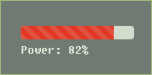
\includegraphics{./img/power-indicator.png}
		\caption{The on-screen power indicator}
		\label{power-indicator}
	\end{figure}
	\subsection{Structure Selection}
	At the start of the game, there is a full pool of pre-defined structures. At the start of each round, a random structure is selected then removed from the pool, meaning no structure can be played twice within the same game. The chosen structure for a given round is initialized twice, allowing both the Human Player and AI Player to take their turn against the same structure.
	\subsection{Calculating Score}
	A score is awarded to the player at the end of their turn. The score is based on how successfully the player 'destroyed' the structure, the more individual blocks the player is able to displace, the higher their score. Scores typically range from 0-150 and a score display is updated after each turn.
	\subsection{AI Player and Difficulty}
	The AI Player, known as 'BOT' within the game has two strategies for attempting to destroy the structure: aiming for the structure's center or aiming for the structure's foundation. The AI Player analyses the current structure to decide which strategy to use. If the structure is tall, the AI chooses the first strategy, otherwise, it chooses the second strategy. The AI Player will always attempt to apply full power to the projectile; however, in order to preserve gameplay, a set error is applied to the projectile's power and direction. 
	
	The AI Player's error value is decided by the game's difficulty, which is chosen by the user at the start of the game (see Fig.~\ref{start-screen}). Each difficulty maps onto a specific error value which is then applied to all of the AI Player's decisions.

	\subsection{Rounds and Turn Alternation}
	In order to give the game a progressive structure, it is broken up into 3 rounds, wherein each player takes their turn - starting with the Human Player. A new round is entered after the AI Player has completed its turn. Once 3 rounds have been played the game finishes and the player is the scores and is given the option to play again or return to the start menu.
	
	\section{Design and Implementation} \label{implementation}
	This section will look in detail at the design and implementation of the functionalities outlined in Section \ref{functionalities}, along with the overall design of the system. 
	\subsection{System Architecture}
	The application implements the revealing module design pattern~\cite{ref_revealing-module-pattern}. A modular codebase is very beneficial to the game's implementation, it allows specific elements of the system to be separated, ultimately making maintenance and adaptation much easier. Implementing the revealing module pattern ~\cite{ref_revealing-module-pattern} also limits the use of the global scope and encourages good encapsulation. The application is split into 5 modules: 
	\begin{itemize}
		\item \textbf{Game} - Handles all of the game logic 
		\item \textbf{Opponent} - Handles the opponent's behaviour
		\item \textbf{Three} Components - Handles all three.js scene objects (camera, lights, meshes, textures, etc.)
		\item \textbf{UI} - Handles the UI components of the game (power indicator, score display, etc.)
		\item \textbf{User Input} - Handles all user input (button presses, mouse movement, etc.)
	\end{itemize}
	\subsection{Screens}
	A finite-state machine (see Fig.~\ref{fsm}) handles all of the game's screens, each screen is tied to a specific state; therefore, only one screen can be shown at any given time. Using a finite-state machine also means that behaviour specific to a screen can only be executed when in the associated state.
	
	The finite-state machine is implemented in the Game module using a variable to store the current state and a function to change state. Changing the state using a function, as opposed to simply changing the variable allows behaviour to be tied to state changes.
	\newpage
	\begin{figure}
		\centering
		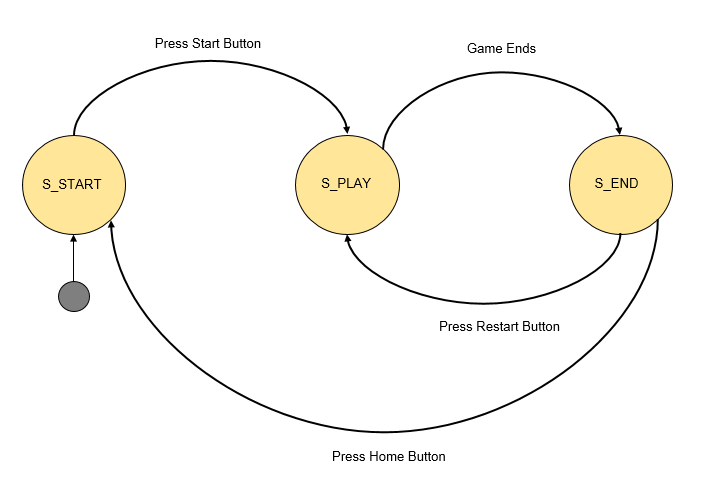
\includegraphics[width=\textwidth]{./img/fsm.png}
		\caption{The finite-state machine that handles all game screens}
		\label{fsm}
	\end{figure}
	\subsection{Firing the Projectile}
	\subsection{Structure Generation}
	\subsection{Calculating Score}
	\subsection{AI Player and Difficulty}
	\subsection{Turn Alternation}
	
	\section{User Interface}
	\section{Review/Evaluation}
	
	\newpage
	\begin{thebibliography}{8}
		\bibitem{ref_threejs}
		Threejs Homepage, https://threejs.org/. Last accessed 15 Nov 2018
		\bibitem{ref_physijs}
		Physijs Project Page, http://chandlerprall.github.io/Physijs/. Last accessed 15 Nov 2018
		\bibitem{ref_revealing-module-pattern}
		Chris Heilmann's Revealing Module Pattern Blog Post, https://christianheilmann.com/2007/08/22/again-with-the-module-pattern-reveal-something-to-the-world/. Last accessed 15 Nov 2018
	\end{thebibliography}
\end{document}